\documentclass[]{iat}
%Diese Beiden Pakete werden nur für das Beispieldokument benötigt und sollten von Ihnen gelöscht werden
\usepackage{listings}
\usepackage{scrhack}
%Hier können weitere benötigte Pakete Eingebunden werden

%Namen eingeben / Insert Name
\renewcommand{\author}{Dasanayake Mudiyanselage Hasith Thilanka Dasanayake}
%Art der Arbeit / Scope (Project, Thesis...)
\providecommand{\scope}{Projektarbeit/Thesis}
%Thema der Arbeit / Theme of Thesis
\renewcommand{\subject}{Thema der Arbeit}
%Schlagwörter / Keywords
\providecommand{\keywords}{Key_1, Key_2}
%Literaturliste *.bib / Bibliography
\providecommand{\bibfile}{IAT_Beispiel_literature}
%Matrikelnummer / Student ID
\providecommand{\studentID}{6003143}
%Betreuer /& Tutors
\providecommand{\tutora}{Stadler}
\providecommand{\tutorb}{Waldorff}
%Prüfer / Examiner
\providecommand{\examinera}{Jekyll}
\providecommand{\examinerb}{Hyde}


\hypersetup{%
	pdftitle	={\subject -- \author -- \today},
	pdfauthor	={\author},
	pdfsubject	={\subject},
	pdfkeywords ={\keywords}
}

\bibliography{\bibfile} 

\setlength{\footheight}{21pt}

\begin{document}
	\lstset{literate={ä}{{\"a}}1}
%Pfad zu Grafiken:
	\graphicspath{{./project_graphics/}}
% Sprachauswahl /Language Selection (ngerman/english)
	\selectlanguage{ngerman}
\pagenumbering{roman}
\begin{titlepage}
\newgeometry{left=0cm,right=0cm,top=0cm,bottom=0cm}
{\color{iatred}\rule{\textwidth}{1cm}}
\begin{minipage}{0.7\textwidth}
	\vspace{-1.37cm}
	{\color{iatred}\rule{\textwidth}{0.5cm}}
\end{minipage}%
\begin{minipage}{0.3\textwidth}
	\raggedright
	\vspace{0.4cm}
	\hspace{0.35cm}
	
\includegraphics[scale=1]{Logos/iat_logo_en}
\end{minipage}%
\centering
\vspace{4cm}

	{\Large
		\textbf{\scope}
	}\par

\vspace{2cm}

    {\linespread{1.1}\huge\sffamily\bfseries
     \subject\par}

\vspace{2cm}

    {\large
     \author\\
     \studentID
    \par}

\vspace{1cm}

	\today
    
\vspace{3cm}
\begin{table}[h]
	\centering
	\begin{tabular}{lll}
		\underline{Betreuer:}	&\quad\hspace{4cm}\quad&\underline{Gutachter:}\hspace{5cm}\\
		\tutora	&	&\examinera\\
		\tutorb	&	&\examinerb
	\end{tabular}
\end{table}
\thispagestyle{empty}  
\vfill
\begin{minipage}{0.3\textwidth}
	\centering
%	\hspace{2cm}
	
\includegraphics[scale=1.2]{Logos/uni_logo_title}\relax
		\vspace{0.1cm}
\end{minipage}%
\begin{minipage}{0.7\textwidth}
	\raggedleft
	{\color{iatred}\rule{\textwidth}{0.5cm}}
	\vspace{-0.9cm}
\end{minipage}
{\color{iatred}\rule{\textwidth}{1cm}}
\end{titlepage}

%Urherberrechtserklärung / Confirmation of Conformity Comment if not needed, Select correct Language
\chapter*{Urheberrechtliche Erklärung}
\thispagestyle{iat-conformity}
Hiermit versichere ich, dass ich meine Abschlussarbeit ohne fremde Hilfe angefertigt habe und dass ich keine Anderen als die von mir angegebenen Quellen und Hilfsmittel benutzt habe.\par
Alle Stellen, die wörtlich oder sinngemä{\ss} aus Veröffentlichungen entommen sind, habe ich unter Angabe der Quellen als solche kenntlich gemacht.\par
Die Abschlussarbeit darf nach der Abgabe nicht mehr verändert werden.\par
\vspace{2.5em}
Datum:\underline{\hspace{3.5cm}}\qquad Unterschrift:\underline{\hspace{5.5cm}}
\vspace{3em}
\section*{Erklärung zur Veröffentlichung von Abschlussarbeiten}
$\Box$ Ich bin damit einverstanden, dass meine Abschlussarbeit im Universitätsarchiv für wissenschaftliche Zwecke von Dritten eingesehen werden darf.\par
$\Box$ Ich bin damit einverstanden, dass meine Abschlussarbeit nach 30 Jahren (gem. §7 Abs.2 BremArchivG) im Universitätsarchiv f`ür wissenschaftliche Zwecke von Dritten eingesehen werden darf.\par
$\Box$ Ich bin \textit{nicht} damit einverstanden, dass meine Abschlussarbeit im Universitätsarchiv für wissenschaftliche Zwecke von Dritten eingesehen werden darf.\par
\vspace{2.5em}
Datum:\underline{\hspace{3.5cm}}\qquad Unterschrift:\underline{\hspace{5.5cm}}

\pagestyle{iat}
\tableofcontents
\chapter{Einleitung / Introduction}
\pagenumbering{arabic}
\setcounter{page}{1}
Dies ist die IAT-Vorlage für Arbeiten in der AG Michels. Das Layout und diverse Einstellungen sind bereits fertig konfiguriert, so dass direkt mit dem Schreiben begonnen werden kann. Für Fragen, Latex-Pakete und Hilfen sei auf\\
\url{https://ctan.org/?lang=de} verwiesen. \par
This is the IAT template for reports at the IAT/Michels research group. The layout and various settings are already configured, so you can start writing right away. For questions, additional packages and help see:\\
\url{https://ctan.org/?lang=en}

\section{Voraussetzungen / Prequisites}
Es muss eine Latex-Distribution (Texlive etc.) installiert sein, ein Editor (Texstudio/MikTex/Vim/Emacs) wird benötigt.
\par
A latex distribution (Texlive etc.) must be installed, an editor (Texstudio/MikTex/Vim/Emacs) is required.

\chapter{Basisbefehle im Textsatz / Basic Controls for Textset}
\section{Strukturieren von Dokumenten / Structure of Documents}
Im Folgend sind die Strukturebenen des Textsatzes von oben nach unten dargestellt.\\
The follows shows the structural levels of the text set top-down:

\boxed{
\begin{minipage}[]{\textwidth}
	\chapter*{Kapitel / Chapter}
	\section*{Abschnitt / Section}
	\subsection*{Unterabschnitt / Subsection}
	\subsubsection*{Unterunterabschnitt / Subsubsection}
	\paragraph{Absatz / Paragraph}
	\quad
\end{minipage}
}
Leerzeilen werden mit \textbackslash\textbackslash\space eingefügt, ein neuer Paragraph ohne Überschrift mit \textbackslash par.\\
To insert a newline type \textbackslash\textbackslash, a new paragraph without title is set with \textbackslash par.

\section{Gleichungen / Equations}
Für das Darstellen von Gleichungen das amsmath-Paket verwenden, z.B. mithilfe der align-Umgebung:\\
Use the amsmath-package for equations, for example the align-environment:
\begin{lstlisting}
\begin{align}
	S(s)&=1-T(s)
\intertext{Beispielgleichung}
	T(s)&=\frac{GK(s)}{GK(s)+1}
\end{align}
\end{lstlisting}
Ergebnis / Result:\par
\begin{align}
	S(s)&=1-T(s)
	\intertext{Beispielgleichung}
	T(s)&=\frac{GK(s)}{GK(s)+1}
\end{align}

Für Einheiten das siunitx-Paket benuten. Z.B.: $v$ in $\si{\m\per\s}$\\
Use the siunitx-package for unit typesetting. E.g.: $v$ in $\si{\m\per\s}$\par
\section{Grafiken / Graphics}
Wenn möglich, Vektorgrafiken verwenden und schwarz/weiß kompatible Grafiken erstellen. Grafiken in figure-Umgebung einbetten. Anstelle die Position mit der Option [h!] oder [H] zu verändern, bis zum Abschluss des Dokumentes warten und, falls noch immer notwendig, mit Clearpage arbeiten oder mit FloatBarrier erzwingen. Im Text kann auf Grafiken mit z.B. autoref aus dem hyperref Paket referenziert werden. In \autoref{fig:exgraph} ist eine Beispielgrafik dargestellt.\par

If possible, use vector graphics and create black and white compatible graphics. Embed graphics in figure environments. Instead of changing the position with the [h!] or [H] option, wait until the document is finished and, if still necessary, work with Clearpage or force the positioning with FloatBarrier. For references to graphics, use e.g. autoref from the hyperref package. An example graphic is shown in \autoref{fig:exgraph}.
\begin{lstlisting}
\begin{figure}[h]
	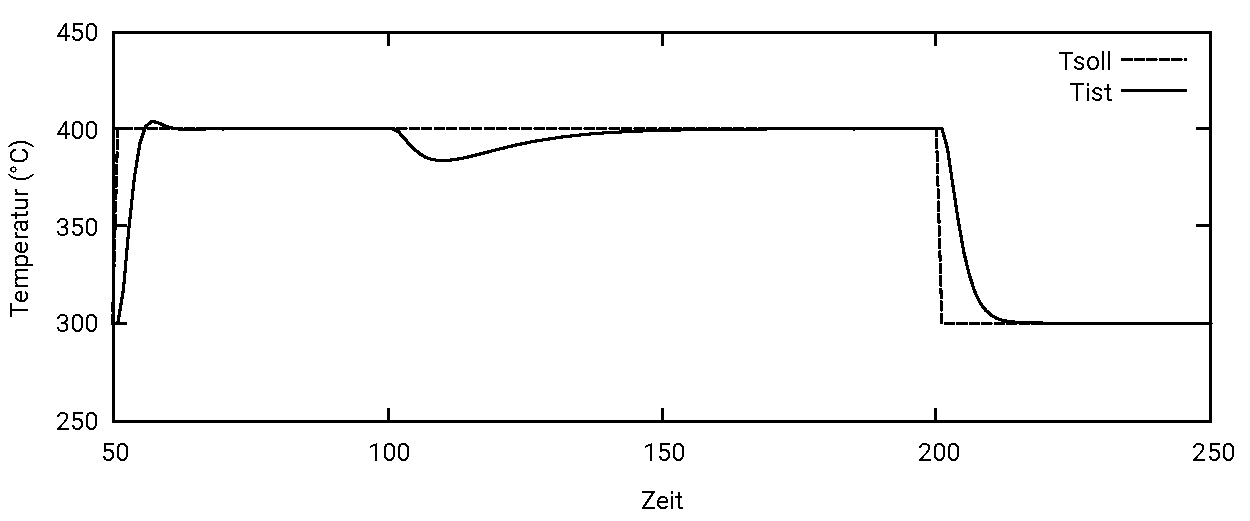
\includegraphics[width=\textwidth]{beispielgrafik}
	\caption{Beispielgrafik mit Unterschrift}
	\label{fig:exgraph}
\end{figure}
\end{lstlisting}
Führt zu / Gives:
\begin{figure}[h]
	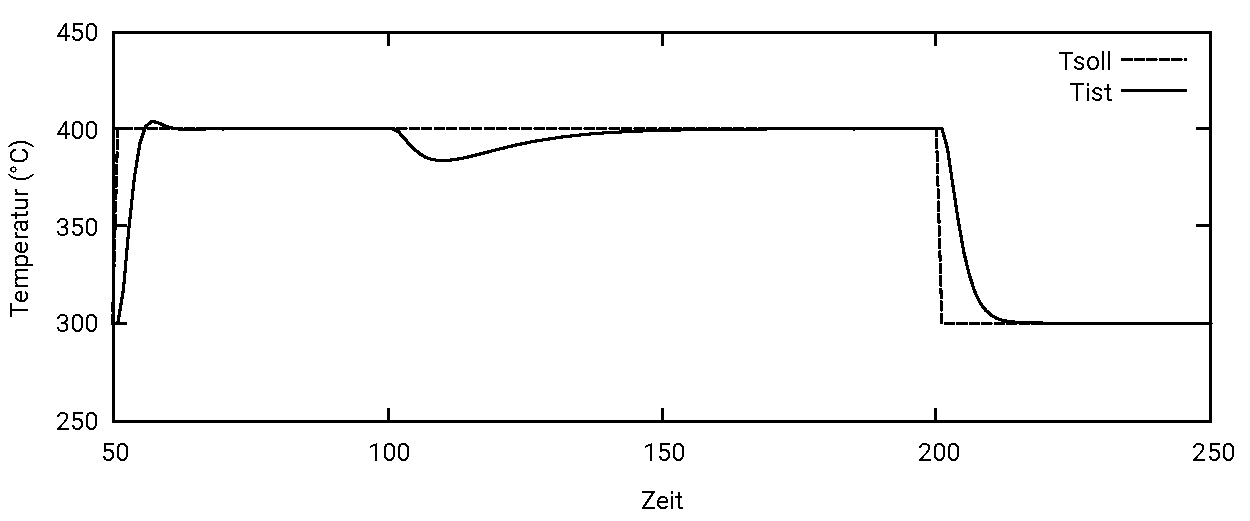
\includegraphics[width=\textwidth]{beispielgrafik}
	\caption{Beispielgrafik mit Unterschrift}
	\label{fig:exgraph}
\end{figure}
\section{Tabellen / Tables}
Für Tabellen ist aus typografischer Sicht folgendes sinnvoll:
\begin{itemize}
	\item möglichst keine vertikalen Linien verwenden
	\item horizontale Linien (\textbackslash hline) sparsam einsetzen
	\item mehrzeiligen Text in Zellen vermeiden
\end{itemize}
Ein Beispiel ist in \autoref{tab:Tabellenbeispiel} abgebildet.
\par
You can create well arranged tables with the following:
\begin{itemize}
	\item avoid vertical lines
	\item use a few horizontal lines (\textbackslash hline)
	\item avoid multiline text in cells
\end{itemize}
An example is shown in \autoref{tab:Tabellenbeispiel}
\par
\begin{lstlisting}
\begin{table}[h]
\begin{tabular}{crl}
	\hline
	Nr.	& Name	& Email			\\\hline
	1	& Max	& max@uni-bremen.de	\\
	2	& Moritz& moritz@uni-bremen.de	\\
	3	& Hermes& hermes@goetterbote.de	\\\hline
\end{tabular}
\caption{Beispiel einer einfachen Tabelle}
\label{tab:Tabellenbeispiel}
\end{table}
\end{lstlisting}
\begin{table}[h]
	\begin{tabular}{crl}
		\hline
		Nr.	& Name	& Email			\\\hline
		1	& Max	& max@uni-bremen.de	\\
		2	& Moritz& moritz@uni-bremen.de	\\
		3	& Hermes& hermes@goetterbote.de	\\\hline
	\end{tabular}
	\caption{Beispiel einer einfachen Tabelle}
	\label{tab:Tabellenbeispiel}
\end{table}

\section{Zitate / Citation}
Es muss ein Literaturverzeichnis mit der Endung .bib angelegt werden (wird durch den Vorlagengenerator im Arbeitsverzeichnis erstellt). Zitate können z.B. mit dem Kommando cite eingefügt werden. Das Biblatex-Biber backend verwenden. Bespiel : \cite{vdi} ist eine gute Quelle im Bereich der thermischen Verfahrenstechnik.\par
A bibliography has to be created with the file extension .bib ( already created by the template generator in the working directory). Quotations can be inserted with the command cite, for example. Use the Biblatex-biber backend. Example : \cite{vdi} is a good source in the field of thermal engineering.
\begin{lstlisting}
	\cite{vdi}
\end{lstlisting}
.bib Beispiel / Example:
\begin{lstlisting}
@BOOK{vdi,
	TITLE	=	{VDI-Wärmeatlas},
	AUTHOR	=	{Verein-Deutscher-Ingenieure},
	DOI	=	{10.1007/978-3-642-19981-3},
	YEAR	=	{2013},
	VOLUME	=	{11},
	PUBLISHER=	{Springer}
}

\end{lstlisting}
\section{Kompilieren / Compilation}
Editoren wie TeXstudio haben vorbereitete Tools für das Erzeugen des Dokumentes und des Literaturverzeichnisses. Im Terminal kann z.B. mit:\\
Editors like TeXstudio have prepared tools for the creation of the document and the bibliography. In the terminal you can use e.g.:
\begin{lstlisting}
	pdflatex <MainDocument.tex>
	biber <MainDocument.tex>
	pdflatex <MainDocument.tex>
\end{lstlisting}
Ein Pdf-Dokument mit Literaturverzeichnis erstellt werden.\\
A Pdf document with bibliography can be created.
\printbibliography
\end{document}
